\sect{5 \quad Why does the Latvian system miss visible scab?}
\subt{Separate the updated prediction from the decision to send}
We hold the camera, cloud expert, image identities and per-image JPEG costs fixed within each counterfactual. This diagnostic uses the retrospective 25\% ceiling and charges 166,798 bytes for the update with available labels. Of 983 scab-positive photographs, the released camera misses 118. The Cornell-trained head alone misses 471.80 on average. Reviewing its uncertain predictions with the PlantDoc expert increases misses to 536.35. Thus 353.80 of the 418.35 additional misses (84.6\%) occur before routing. On the transmitted set the server rescues 25.50 misses and introduces 90.05. It removes 25.95 false positives and introduces 1.50. Total false alarms fall from 195 to 74.45. BA thus rises from 46.90\% to 54.74\% even while ordinary accuracy falls from 73.70\% to 48.67\%. The selected camera decisions are correct on 53.66\% of sent images, the cloud's replacements on 38.92\%.

\begin{center}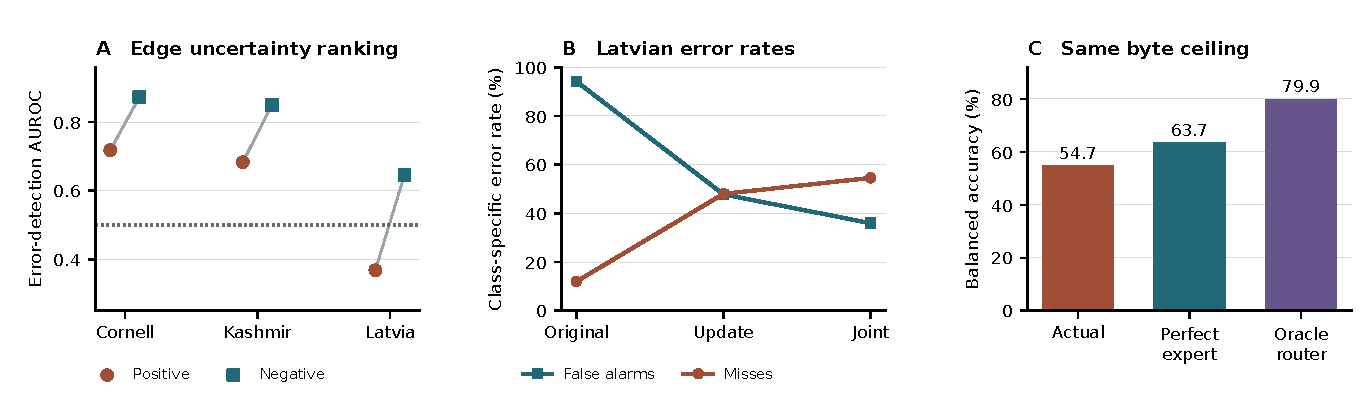
\includegraphics[width=.97\linewidth]{figures/latvia_failure.pdf}\end{center}
\note{Figure 1. Error-detection AUROC conditions on the indicated true class. The stage counts identify when additional misses occur. The label-aware routing ceiling holds both classifiers and the byte allowance fixed. Its access to truth makes it an unattainable deployment reference.}

\subt{A changed endpoint and a changed source}
Cornell's negative class is explicitly healthy. Latvia's negative class means no visible scab and can contain other damage. Restricting Cornell to its 450 scab and 377 healthy evaluation images brings the positive endpoints closer. The updated head's disease-score AUROC is 0.905 on this restriction and 0.528 on Latvia. The frozen server gives 0.955 and 0.696. Changing the positive prevalence alone cannot produce this within-class ranking loss. Restricting Latvian comparisons to positive--negative pairs from the same camera model and date gives edge AUROC 0.512 and cloud AUROC 0.666, covering 8.38\% of possible pairs across eleven mixed strata. We lack common independent labels for scab and any disease on the same Latvian leaves. Acquisition, orchard, severity and residual endpoint differences therefore remain confounded.

Uncertainty detects errors on positive Latvian leaves with AUROC 0.368. It assigns higher priority to many correct positive calls than to misses. At the same cost, a truth-aware router selecting among the actual edge and cloud answers could reach 79.95\% BA, versus 54.74\% for the margin. After removing near-duplicates, margin and random uploads give 54.570\% and 54.526\%, respectively. This is a failure of the available ranking and the expert on its selected cases, even though some affordable frames could have been repaired.

\newpage
\subt{Resolution and site-specific heads}
Keeping the DINO weights, threshold and crop rule fixed, we decoded all 1,190 images from each candidate payload. Full-review AUROC improves from 0.696 at 224 pixels to 0.743 at 448 and 0.757 using the original camera files. Even the latter yields 637 missed scab cases. With the original query identities, the camera--cloud BA improves from 54.74\% to 55.72\% and 55.79\%. With the original \emph{byte} allowance, however, 448 pixels admits 90.5 queries instead of 271.8, lowering BA to 53.30\%. Camera originals admit one query on average and give 52.14\%. This intervention holds the trained classifier fixed and separates loss of visual information from the price of sending it.

We also fit separate edge and server heads using the same 128 early Latvian labels per draw and evaluate only the 579 later images (507 scab, 72 negative). The 25\% inference allowance is identical and setup is prepaid to isolate each component. In the table, the two entries for a given edge head use exactly the same query identities.
\begin{center}\small
\begin{tabular}{@{}llrrr@{}}\toprule
Edge head & Server head & False alarms & Misses & BA (\%)\\\midrule
Cornell & PlantDoc & 23.80 & 267.80 & 57.06\\
Cornell & Early Latvia & 29.70 & 216.65 & 58.01\\
Early Latvia & PlantDoc & 37.35 & 201.40 & 54.20\\
Early Latvia & Early Latvia & 42.35 & 146.70 & 56.12\\\bottomrule
\end{tabular}\end{center}
With every later image reviewed, refitting the server raises its BA from 63.09\% to 68.11\%. Changing both heads brings down missed cases but increases the false alarms among the 72 negatives. The small number of negative dates limits extrapolation to other seasons.

\sect{6 \quad Device and link sensitivity}
\subt{From exported FP32 features to the released INT8 scales}
We replayed the model's recorded ESP-PPQ tensor scales on the CPU using signed quantization and the S3 rounding rule \cite{esp}. For the embedded fixture the host gives output codes $(56,-62)$ versus $(58,-59)$ in the release. It matches 59 of 60 archived binary board decisions, with median absolute disease-probability difference 0.000172 and a maximum of 0.204. This measures numerical sensitivity rather than certifying hardware parity.

On the three evaluation cohorts, median cosine similarity between approximate INT8 and FP32 features is 0.894, 0.908 and 0.918. Holding the FP32-fitted head fixed gives joint BA of 78.86\%, 77.73\% and 50.39\% under remote annotation and the retrospective 25\% ceiling. The FP32 reference gives 84.76\%, 76.37\% and 53.70\%. Retraining the heads on the simulated activations gives 81.60\%, 77.73\% and 53.26\%. For Kashmir the update cannot fit and these comparisons use their respective frozen-camera fallbacks. The approximation can therefore shift predictions enough to affect the operating recommendation. Deployed feature tensors and the latency, total RAM and energy of the new head on an ESP32-S3 remain unmeasured.

\newpage
\subt{An alert deadline changes the value of sending an image}
We distinguish link measurements from assumed operating conditions. Nine public Norwegian forest private-5G measurements provide average uplink goodput (8--179 Mbit/s), downlink goodput (133.4--624 Mbit/s) and RTT (12--27 ms) at different distances \cite{forest}. They are snapshots, without packet arrival times. We replay the same byte-selected queries across each snapshot, add one RTT on an existing connection or three for a cold connection, and budget 0.1 or 0.5 s for cloud work. Late replies preserve the local classification. This separately probes delivery of the retrospective selection. The online routing evaluation in Section 3 assumes replies from funded requests are available.

Under remote 128-label setup, the Cornell camera requests 166.4 reviews on average. All arrive within 2 s in the nine snapshot replays with a 5 s acquisition interval. A separate synthetic link runs at 10/20 kbit/s up/down, RTT 1.2 s, independent 10\% segment loss, up to five attempts, and 60 s out of service every 120 s. At a 2 s deadline none return in time (80.01\% BA). With an existing connection, 0.1 s cloud work and a 30 s deadline, 85.0 arrive on time (82.36\% BA), compared with 84.76\% if every requested reply counts. Expert time is additional: at assumed sequential service of 15 or 60 s per calibration image, 128 labels require 32 or 128 minutes of labor. The link and time assumptions are sensitivities; none is a new measurement from an orchard, an NB-IoT carrier or a human annotator.

\sect{7 \quad What the evidence supports}
For an operator who must send calibration photographs, 32 labels used the nominal online allowance more effectively than 128 in Kashmir, whereas 128 gave the largest of the two mean scores in Cornell. A separate exact cost comparison on Cornell asks how much a truth-aware router must spend to match the updated head alone. The update costs 166,798 bytes with all 128 labels already available, versus 1,026,890 on average when all 128 photographs must be sent. The update is cheaper in 20/20 draws with local labels, 9/20 when 32 of the 128 photographs must be sent, and 0/20 from 64 sent onward in this nested comparison. This bound is specific to the fixed menu in Appendix C. The answer depends on the camera's starting classifier as well as annotation access.

The binary uncertainty score has the same ordering as EdgeBoost with a positive temperature. Matched learned alternatives and a simple cross-entropy control can equal or improve on its results. Across sources, the updated camera assigns low uncertainty to many scab-positive images it misses. The study's contribution is a reproducible set of cost and failure comparisons. The experiments neither establish a superior general routing algorithm nor verify an end-to-end field deployment. A matched dual-label reannotation and board-side feature capture would be needed to identify the remaining endpoint and hardware effects.
